\chapter[转动动力学]{\itr{Rotation Dynamics}{转动动力学}}
\begin{prove}[Concepts in Dynamics\qquad$\vec{\tau}_{net}=I\vec{\alpha}$]
	要搞清楚的一点是,我们依旧基于牛顿力学来思考有关转动的问题。
	
	我们先承认一件事实:刚体的内部存在着非常复杂的相互作用力,这些作用力合理地分配,最终使得整个刚体可以做转动。于是,任意取一个质元$\dif m$分析,都有\[\dif \vec{F}_t=\dif m\vec{a}_t\]
	
	依据平动和转动的联系(见\refleaftext{chapter3_connection}),我们有
	\[\vec{a}_t\dif m=(\vec{\alpha}\times\vec{r})\dif m\]
	于是在等式两侧同左叉乘以$\vec{r}$,即有
	\[\vec{r}\times\dif\vec{F}_t= (\vec{r}\times\vec{\alpha}\times\vec{r})\dif m\]
	由双重叉乘的运算律(见\refleaftext{chapter3_double_cross_product}),知
	\[\vec{r}\times\vec{\alpha}\times\vec{r}=(\vec{r}\cdot\vec{r})\vec{\alpha}-(\vec{\alpha}\cdot\vec{r})\vec{r}=r^2\vec{\alpha}\]
	注意到
	\[\vec{r}\times\dif\vec{F}_t=\vec{r}\times\dif\vec{F}_{/z}\]
	即得
	\[\vec{r}\times\dif\vec{F}_{/z}=r^2\vec{\alpha}\dif m\Leftrightarrow\dif\vec{\tau}=r^2\vec{\alpha}\dif m\]
	等式两侧取积分,即有
	\[\vec{\tau}_{net}=I\vec{\alpha}\]
\end{prove}
%\refleaf*{chapter3_connection}[-64ex]
%\refleaf*{chapter3_double_cross_product}[-40ex]
%\newpage
\newpage
\begin{prove}[\itr{Parallel Axis Theorem}{平行轴定理}\qquad$I=I_{CM}+Mh^2$]
	不妨设$\vec{h}$的方向为从质心轴到任意轴,并取任意一质点$m_i$,其在选择质心轴时,位矢为$\vec{r}_{CMi}$,选择任意轴时,位矢为$\vec{r}_i$,则有\[\vec{r}_i=\vec{r}_{CMi}-\vec{h}\]
	于是有
	\begin{align*}
		I&=\sum_{i}m_i(\vec{r}_{CMi}-\vec{h})^2\\
		&=\sum_{i}m_i(r_{CMi}{}^2+h^2-2\vec{r}_{CMi}\cdot\vec{h})\\
		&=\sum_{i}m_ir_{CMi}{}^2+\sum_{i}m_ih^2-2\vec{h}\cdot\sum_{i}m_i\vec{r}_{CMi}\\
		&=I_{CM}+Mh^2+0\qquad(\text{由质心的性质知最后一项为0})\\
		&=I_{CM}+Mh^2
	\end{align*}
\end{prove}
\begin{prove}[Energy in Rotation ONLY]
	在只发生转动的物体中,有\[v=v_t=\omega r\]于是有
	\begin{align*}
		K_R&=\sum_i\dfrac{1}{2}m_iv_i{}^2&U&=\int_0^{\theta}\kappa\alpha\dif\alpha\\
		&=\sum_i(\dfrac{1}{2}m_i r_i{}^2)\omega^2&&=\dfrac{1}{2}\kappa\alpha^2\left|_0^{\theta}\right.\\
		&=I\omega^2&&=\dfrac{1}{2}\kappa\theta^2\\
		P&=\vec{F}\cdot \vec{v}&\dif W&=\vec{F}\cdot\dif \vec{x}\\
		&=F_tv&&=F_t\dif x\\
		&=F_tr_\omega&&=F_tr\dif\theta\\
		&=\tau\omega&&=\tau\dif\theta
	\end{align*}
\end{prove}
%\newpage
\begin{prove}[\itr{Konig's Theorem}{柯尼希定理}\qquad$K=K_{CM}+K^{CM}$]
	我们取质点$m_i$,记它在静止参考系中的速度为$\vec{v}_i$,在质心系中的速度为$\vec{v}^{CM}_i$,并记刚体的质心速度为$\vec{v}_{CM}$,则有
	\[\vec{v}_i=\vec{v}_i^{CM}+\vec{v}_{CM}\]
	于是有
	\begin{align*}
		K&=\sum_i\dfrac{1}{2}m_i(\vec{v}_i^{CM}+\vec{v}_{CM})^2\\
		&=\sum_i\dfrac{1}{2}m_i{v_i^{CM}}^2+\sum_i\dfrac{1}{2}m_i{v_{CM}}^2+(\sum_im_i\vec{v}_i^{CM})\cdot\vec{v}_{CM}\\
		&=K^{CM}+K_{CM}\qquad(\text{由质心定义知前式最后一项为0})
	\end{align*}
	由刚体在质心系中只存在转动(见\refleaftext{chapter3_rotation_CM}),有
	\[K^{CM}=\dfrac{1}{2}I_{CM}\omega^2\]
	于是
	\[K=\dfrac{1}{2}M{v_{CM}}^2+\dfrac{1}{2}I_{CM}\omega^2\]
\end{prove}
%\refleaf*{chapter3_rotation_CM}[-22ex]
%\newpage
\begin{prove}[Angular Momentum\qquad$\displaystyle\vec{L}=\sum_i\vec{r}_i\times\vec{p}_{i/z}=I\vec{\omega}\quad\&\quad\dfrac{\dif \vec{L}}{\dif t}=\vec{\tau}$]
	\qquad
	$
	\begin{array}{r@{\ }l}
		\vec{L}&=\displaystyle\sum_i\vec{r}_i\times\vec{p}_{i/z}\\
		&=\displaystyle\sum_im_i\vec{r}_i\times(\vec{v}_{ir}+\vec{v}_{it})\\
		&=\displaystyle\sum_im_i(\vec{r}_i\times\vec{v}_{ir}+\vec{r}_i\times\vec{v}_{it})\\
		&=\displaystyle\sum_im_i(\vec{0}+\vec{r}_i\times(\vec{\omega}\times\vec{r}_i))\\
		&=\displaystyle\sum_im_i((\vec{r}_i\cdot\vec{r}_i)\vec{\omega}+(\vec{r_i}\cdot\vec{\omega})\vec{r}_i)\\
		&=\displaystyle\sum_im_ir_i{}^2\vec{\omega}\\
		&=I\vec{\omega}
	\end{array}$有关双重叉乘见\refleaftext{chapter3_double_cross_product}
	\\[2ex]
	\hspace*{0.9em}
	$
	\begin{array}{r@{\ }l}
		\dfrac{\dif\vec{L}}{\dif t}&=\dfrac{\dif\displaystyle\sum_i(\vec{r}_i\times\vec{p}_{i/z})}{\dif t}\\[1.4ex]
		&=\displaystyle\sum_i\dfrac{\dif(\vec{r}_i\times\vec{p}_{i/z})}{\dif t}\\
		&=\displaystyle\sum_i(\dfrac{\dif\vec{r}_i}{\dif t}\times\vec{p}_{i/z}+\vec{r}_i\times\dfrac{\dif\vec{p}_{i/z}}{\dif t})\\
		&=\displaystyle\sum_i(\vec{v}_{i/z}\times\vec{p}_{i/z}+\vec{r}_i\times\vec{F}_{i/z})\\
		&=\displaystyle\sum_i\vec{r}_i\times\vec{F}_{i/z}\\
		&=\vec{\tau}_{net}
	\end{array}$
	有关微分见\refleaftext{chapter3_derivation}
\end{prove}
%\refleaf*{chapter3_double_cross_product}[-62ex]
%\refleaf*{chapter3_derivation}[-23ex]
\begin{prove}[$\vec{L}=\vec{L}_{CM}+\vec{L}^{CM}$]
	我们取质点$m_i$,记它在静止参考系中的速度为$\vec{v}_i$,极径矢量为$\vec{r}_i$在质心系中的速度为$\vec{v}^{CM}_i$,极径矢量为$\vec{r}_i^{CM}$,并记刚体在静止参考系中的质心速度为$\vec{v}_{CM}$,极径矢量为$\vec{r}_{CM}$则有
	\[\vec{v}_i=\vec{v}_i^{CM}+\vec{v}_{CM}\]
	\[\vec{r}_i=\vec{r}_i^{CM}+\vec{r}_{CM}\]
	于是有
	\begin{align*}
		\vec{L}&=\sum_im_i\vec{r}_i\times v_i\\
		&=\sum_im_i(\vec{r}_i^{CM}+\vec{r}_{CM})(\vec{v}_i^{CM}+\vec{v}_{CM})\\
		&=\sum_im_i\vec{r}_i^{CM}\times\vec{v}_i^{CM}+\sum_im_i\vec{r}_{CM}\times\vec{v}_{CM}\\
		&+(\sum_im_ir_i^{CM})\times\vec{v}_{CM}+\vec{r}_{CM}\times(\sum_im_i\vec{v}_i^{CM})\\
		&=\vec{L}^{CM}+\vec{L}_{CM}+\vec{0}\times\vec{v}_{CM}+\vec{r}_{CM}\times\vec{0}\quad(\text{利用质心性质})\\
		&=\vec{L}^{CM}+\vec{L}_{CM}
	\end{align*}
\end{prove}
\newpage
\quad\\
\begin{prove}[\itr{Center of Gravity}{重心}:对于均匀的重力场,刚体的重心与质心重合]
	记重力的合力矩为$\vec{\tau}_{g}$,等效于质心的重力力矩为$\vec{\tau}_{g_{CM}}$,有
	\begin{align*}
		\vec{\tau}_g&=\sum_i\vec{r}_i\times(m_i\vec{g}_{/z})\\
		&=(\sum_im_i\vec{r_i})\times\vec{g}_{/z}\\
		&=M\vec{r}_{CM}\times\vec{g}_{/z}\quad(\text{由质心定义知})\\
		&=\vec{r}_{CM}\times(M\vec{g}_{/z})\\
		&=\vec{\tau}_{g_{CM}}
	\end{align*}
	即刚体重心与质心重合。
	
	在这里的证明中,我们发现,只要一个力仅与质量成正比,方向不变,那么分析力矩时,就可以把这些力等效作用在质点上。
\end{prove}
\begin{comment}
	\begin{prove}[\itr{Frame Translation with Rotation}{考虑转动的参考系变换}]
		我们考虑一个在惯性系$\mathcal{F}_{inertial}$中旋转的参考系$\mathcal{F}_{rotation}$,其原点拥有位矢$\vec{R}_i$,%速度$\vec{v}_i$,加速度$\vec{a}_i$,
		坐标系的$x,y$轴则以角速度$\vec{\omega}$旋转。
		
		此外,我们再考虑一个质点$m$,它在在惯性系$\mathcal{F}_{inertial}$中拥有位矢$\vec{R}$,速度$\vec{v}$,加速度$\vec{a}$。
		
		我们约定,位矢$\vec{R}$可以分解成沿$z$轴的分量$\vec{R}_z$和极径矢量$\vec{r}$,对参考系原点同理有$\vec{R}_i=\vec{R}_{iz}+\vec{r}_i$。
		
		另外,我们再约定微分符号$\mathrm{D}$和$\dif$的区别。我们用$\dfrac{\mathrm{D}\ }{\mathrm{D} t}$表示在惯性系$\mathcal{F}_{inertial}$中对时间的微分,$\dfrac{\dif\ }{\dif t}$表示在旋转系$\mathcal{F}_{rotation}$中对时间的微分。\\[1ex]
		接下来,我们取时间元$\Delta t$,观察质点在$\mathcal{F}_{rotation}$中的位矢$\vec{R}^{f}$将会如何变化。
		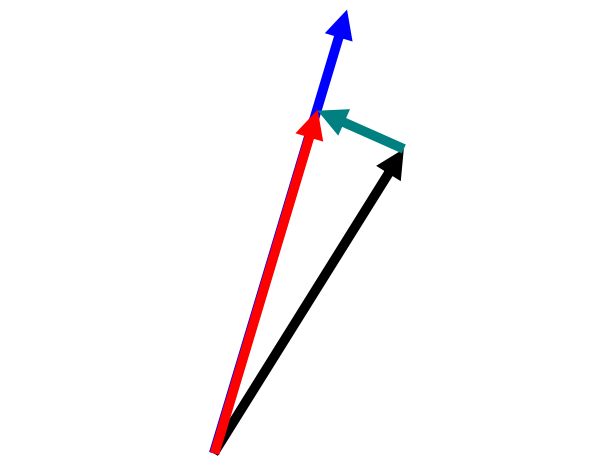
\includegraphics[width=0.45\linewidth]{chapter3_prove_3_8}
		\begin{minipage}[b]{0.5\linewidth}
			\itshape
			在这张示意图中,黑色线条表示当前时刻的$\vec{r}^f$,绿色线条表示在$\dif t$中由于$\mathcal{F}_{rotation}$的旋转导致的极径矢量改变,蓝色线条表示在$\dif t$中由于%$\mathcal{F}_{ratation}$和
			质点的平动导致的极径矢量改变。至于同时因旋转和平动导致的改变,由于是个二阶小量,这里并不画出。
			\vspace{1em}\quad
		\end{minipage}
		
		可以注意到,黑色线条旋转至红色线条产生的夹角为$-\vec{\omega}\Delta t$,且由于该角是个无穷小量,可以认为绿色线条与黑色线条正交,并且,我们还有绿色线条的长度为$r^f\omega\Delta t$。那么,绿色线条恰好可以表示为:
		\[{\color{green!50!black}\Delta\vec{r}}=(-\vec{\omega}\Delta t)\times \vec{r}^f\]
		至于蓝色线条,则可简单地通过平动速度得到:
		\[{\color{blue}\Delta\vec{r}}=\vec{v}_{/z}%-\vec{v}_{f/z})
		\Delta t\]
		求和即得$\Delta t$内质点在$\mathcal{F}_{rotation}$中极径矢量的变化量为
		\begin{align*}
			\Delta\vec{r}^f&={\color{green!50!black}\Delta\vec{r}}+{\color{blue}\Delta\vec{r}}\\
			&=(-\vec{\omega}\Delta t)\times \vec{r}^f+\vec{v}_{/z}-%\vec{v}_{f/z})
			\Delta t\\
			&=(-\vec{\omega}\times\vec{r}^f+\vec{v}_{/z}%-\vec{v}_{f/z}
			)\Delta t
		\end{align*}
		相除即得
		\[\vec{v}_{/z}^f=\dfrac{\Delta \vec{r}^f}{\Delta t}=-\vec{\omega}\times\vec{r}^f+\vec{v}_{/z}%-\vec{v}_{f/z}
		\]
		我们把上式变换形式:
		\begin{align*}
			(\dfrac{\dif\ }{\dif t})\vec{r}=(\dfrac{\mathrm{D}\ }{\mathrm{D} t}-\vec{\omega\times})\vec{r}
		\end{align*}
		
	\end{prove}
\end{comment}
\newcommand{\base}[1]{\hat{\vec{#1}}}
\begin{prove}[\itr{Frame Translation with Rotation}{考虑转动的参考系变换}*]
	这一次,我们采用坐标分解的观点思考问题。
	
	首先,考虑一个惯性系,并建立一个常规的空间直角坐标系$\mathcal{F}$,它的基为$\hat{\vec{i}},\hat{\vec{j}},\hat{\vec{k}}$,即为$x,y,z$轴方向的单位向量(单位向量没有量纲,长度为1)。那么,任取一个质点,它的位矢$\vec{P}$可以表示为\[
	\vec{P}=x\hat{\vec{i}}+y\hat{\vec{j}}+z\hat{\vec{k}}
	\]
	我们另建立一个拥有$x',y',z'$轴的,以角速度$\vec{\omega}$旋转的坐标系$\mathcal{F}'$,其中$z'$轴作为旋转轴与$z$轴平行。设该坐标系原点位矢$\vec{O'}$在原参考系中的表达式为$\vec{O}=x_0\hat{\vec{i}}+y_0\hat{\vec{j}}+z_0\hat{\vec{k}}$,那么在$\mathcal{F}'$中,设
	\[\vec{P}-\vec{O'}=\vec{P}'=x'\hat{\vec{i}'}+y'\hat{\vec{j}'}+z'\hat{\vec{k}'}\]
	如此,我们说,$\vec{P}$在$\mathcal{F}$中的坐标为$(x,y,z)$,在$\mathcal{F}'$中的坐标为$(x',y',z')$。
	
	接下来,我们考虑在不同坐标系中的速度。
	
	$\mathcal{F}$中的速度定义为\[\vec{v}=v_x\base{i}+v_y\base{j}+v_z\base{k}\]其中
	\[v_x=\dfrac{\dif x}{\dif t},v_y=\dfrac{\dif y}{\dif t},v_z=\dfrac{\dif z}{\dif t}\]
	于是
	\begin{align}
		\dfrac{\dif\vec{P}}{\dif t}&=\dfrac{\dif(x\hat{\vec{i}})}{\dif t}+\dfrac{\dif(y\hat{\vec{j}})}{\dif t}+\dfrac{\dif(z\hat{\vec{k}})}{\dif t}\\
		&=\dfrac{\dif x}{\dif t}\hat{\vec{i}}+\dfrac{\dif y}{\dif t}\hat{\vec{j}}+\dfrac{\dif z}{\dif t}\hat{\vec{k}}\\
		&=v_x\hat{\vec{i}}+v_y\hat{\vec{j}}+v_z\hat{\vec{k}}\\
		&=\vec{v}
	\end{align}
	其中由(3.2)到(3.3)的理由是该参考系的基$\hat{\vec{i}},\hat{\vec{j}},\hat{\vec{k}}$始终不变。
	
	同理,$\mathcal{F}'$中的速度定义为
	\[\vec{v}'=v_x'\base{i'}+v_y'\base{j'}+v_z'\base{k'}\]
	其中
	\[v_x'=\dfrac{\dif x'}{\dif t},v_y'=\dfrac{\dif y'}{\dif t},v_z'=\dfrac{\dif z'}{\dif t}\]
	\\[1ex]
	由$\vec{P}'=\vec{P}-\vec{O'}$,且$\vec{O}'$不变,知$\dfrac{\dif \vec{P'}}{\dif t}=\dfrac{\dif\vec{P}}{\dif t}=\vec{v}$。于是有
	\begin{align}
		\vec{v}&=\dfrac{\dif\vec{P}'}{\dif t}\\
		&=\dfrac{\dif(x'\hat{\vec{i}'})}{\dif t}+\dfrac{\dif(y'\hat{\vec{j}'})}{\dif t}+\dfrac{\dif(z'\hat{\vec{k}'})}{\dif t}\\
		&=\dfrac{\dif x'}{\dif t}\hat{\vec{i}'}+\dfrac{\dif\hat{\vec{i}'}}{\dif t}x'+\dfrac{\dif y'}{\dif t}\hat{\vec{j}'}+\dfrac{\dif\hat{\vec{j}'}}{\dif t}y'+\dfrac{\dif z'}{\dif t}\hat{\vec{k}'}+\dfrac{\dif\hat{\vec{k}'}}{\dif t}z'
	\end{align}
	注意到
	\[\dfrac{\dif\base{i'}}{\dif t}=\vec{\omega}\times\base{i'},\dfrac{\dif\base{j'}}{\dif t}=\vec{\omega}\times\base{j'}\]
	续(3.7)有
	\begin{align}
		\vec{v}&=v_x'\base{i'}+v_y'\base{j'}+v_z'\base{k'}+\vec{\omega}\times\base{i'}x'+\vec{\omega}\times\base{j'}y'\\
		&=\vec{v}'+\vec{\omega}\times\vec{r}'\qquad(\text{这里记}\vec{r}'=x'\base{i'}+y'\base{j'})
	\end{align}
	关于加速度,我们有类似的定义
	\[\left\{\begin{array}{c}
		\vec{a}=a_x\base{i}+a_y\base{j}+a_z\base{k}\\[1ex]
		a_x=\dfrac{\dif v_x}{\dif t},a_y=\dfrac{\dif v_y}{\dif t},a_z=\dfrac{\dif v_z)}{\dif t}
	\end{array}
	\right.\]
	\[\left\{\begin{array}{c}
		\vec{a}'=a_x'\base{i'}+a_y'\base{j}'+a_z'\base{k'}\\[1ex]
		a_x'=\dfrac{\dif v_x'}{\dif t},a_y'=\dfrac{\dif v_y'}{\dif t},a_z'=\dfrac{\dif v_z'}{\dif t}
	\end{array}
	\right.
	\]
	对(3.9)左右两侧同时对时间微分,有
	\begin{align}
		\mathrm{LHS}&=\dfrac{\dif\vec{v}}{\dif t}\\
		&=\dfrac{\dif v_x}{\dif t}\base{i}+\dfrac{\dif v_y}{\dif t}\base{j}+\dfrac{\dif v_z}{\dif t}\base{k}\\
		&=\vec{a}
	\end{align}
	\begin{align}
		\mathrm{RHS}&=\dfrac{\dif\vec{v}'}{\dif t}+\dfrac{\dif(\vec{\omega}\times\vec{r}')}{\dif t}\\
		&=\dfrac{\dif(v_x'\base{i}')}{\dif t}+\dfrac{\dif(v_y'\base{j}')}{\dif t}+\dfrac{\dif(v_z'\base{k}')}{\dif t}+\dfrac{\dif\vec{\omega}}{\dif t}\times\vec{r}'+\vec{\omega}\times\dfrac{\dif\vec{r}'}{\dif t}\\
		&=\vec{a}'+\vec{\omega}\times(v_x'\base{i'}+v_y'\base{j'})+\vec{\alpha}\times\vec{r}'+\vec{\omega}\times\dfrac{\dif\vec{r}'}{\dif t}
	\end{align}
	记$v_x'\base{i'}+v_y'\base{j'}=\vec{v}_{/z}'$,则续(3.15)有
	\begin{align}
		\mathrm{RHS}&=\vec{a}'+\vec{\omega}\times\vec{v}_{/z}'+\vec{\alpha}\times\vec{r}'+\vec{\omega}\times(\vec{v}_{/z}'+\vec{\omega}\times\vec{r}')\\
		&=\vec{a}'+2\vec{\omega}\times\vec{v}_{/z}'+\vec{\alpha}\times\vec{r}'-\omega^2\vec{r}'
	\end{align}
	这里注意到$\vec{\omega}\times\vec{v}_{/z}'=\vec{\omega}\times\vec{v}'$,因为$\vec{v}_z'$与$\vec{\omega}$平行。
	
	于是将左式与右式联立,得
	\[\vec{a}'=\vec{a}-2\vec{\omega}\times\vec{v}'-\vec{\alpha}\times\vec{r}'+\omega^2\vec{r}'\]
	其中(3.16)$\Rightarrow$(3.17)有关双重叉乘见\refleaftext{chapter3_double_cross_product}
	
	两侧同时乘以$m$,即得牛顿第二定律形式
	\[m\vec{a}'=m\vec{a}-2m\vec{\omega}\times\vec{v}'-m\vec{\alpha}\times\vec{r}'+m\omega^2\vec{r}'\]
	这意味着,如果希望牛顿运动定律在$\mathcal{F}'$中依然成立,我们需要对$\mathcal{F}'$中的物体添加三个假想力,分别是$-2m\vec{\omega}\times\vec{v}',\quad-m\vec{\alpha}\times\vec{r}',\quad m\omega^2\vec{r}'$。
	
	如果我们将条件简化,认为$\mathcal{F}'$没有角加速度,则有
	\[m\vec{a}'=m\vec{a}-2m\vec{\omega}\times\vec{v}'+m\omega^2\vec{r}'\]
	当$\mathcal{F}'$还拥有平动速度,平动加速度时,只需依照矢量叠加原理分析,再添上惯性力,牛顿第二定律就能继续保持成立。
\end{prove}